\section*{Preface}
\addcontentsline{toc}{subsection}{Preface}

The Large Synoptic Survey Telescope (LSST) is an astronomical sky
survey designed to image $25000\square\degree$ of the sky (including
the entire southern hemisphere) in 6 different filters, repeatedly for
10 years. Such a data set will allow creation not only of a catalog of
objects in the covered area, but also the generation of light curves
of variable objects in the covered area. The LSST Dark Energy Science
Collaboration (DESC) formed to advise the LSST project on optimizing
the survey for cosmology, and prepare for and perform cosmological
analysis on this data set.

In the summer of 2018, the LSST project issued a call for white papers
to provide input on the effects of cadence and other survey strategy
considerations on science. This call was accompanied by the release of
a set of simulated surveys generated using different strategies. The
DESC constituted an Observing Strategy Task-Force to organize
responses to this call. Different analysis working groups within the
DESC developed metrics to evaluate simulated surveys for effectiveness
for different kinds of analysis, and measured these metrics against
the simulations with call for white papers, and others.

The call for white papers specified a specific structure for the
responses, and placed tight limits on their length. On the other hand,
the extensive work carried out by the DESC OSTF and analysis working
groups requires significant documentation to recond and explain, and
different levels of detail and refinement are suitable for different
audiences. The OSTF has therefore developed ``wedding cake'' approach
to documenting the strategy evaluation work; see
figure~\ref{fig:weddingcake}.

\begin{figure}[here]
  \centering
  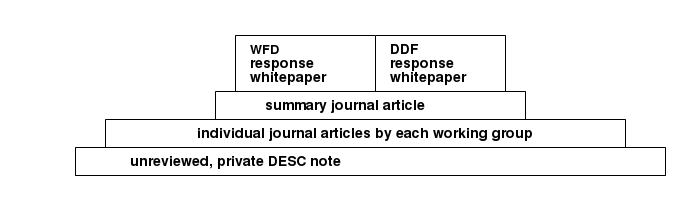
\includegraphics[width=0.75\columnwidth]{wedding_cake.png}
  \caption{The ``wedding-cake'' documentation scheme}
  \label{fig:weddingcake}
\end{figure}

Each level of the wedding cake represents a set of documents at
different levels of detail, intended for different audiences.

\begin{description}
  \item[response white papers] summarize the priorities of the DESC
    for the WFD and DDF programs, respectively. These documents follow
    the specification laid out in the LSST project's call for white
    papers, both in structure and length. The primary audience for
    these white papers is the LSST project.
  \item[a summary journal article] summarizes the metrics developed by
    each of the analysis working groups, and presents the results of
    the application of these metrics to the reference simulation
    results. The audience for this article includes both the LSST
    project, and also the astronomical community as a whole.
  \item[individual journal article] written by each of the analysis
    groups provide more detailed descriptions and discussion for
    metrics from each analysis group. Members of the scientific
    community wanting more detail than that presented in the summary
    paper constitute the audience for these articles.
  \item[DESC notes] provide more thorough and immediate documentation
    of the work performed to develop, implement, and apply the metrics
    to simulations. These notes will be dynamic, and not peer
    reviewed. Members of the DESC OSTF and analysis working groups
    themselves are the audience for these documents, which will
    support refinement of the metrics and application of them to
    future simulations.
\end{description}


Two DESC notes (the lowest level of the cake) have been produced:
one analyzing the use of type 1a supernova, and this one, which is a
compilation of the write-ups from the remaining analysis groups.
